\documentclass[a4paper]{amsart}
\usepackage{geometry}                % See geometry.pdf to learn the layout options. There are lots.
\geometry{letterpaper}                   % ... or a4paper or a5paper or ... 
%\geometry{landscape}                % Activate for for rotated page geometry
%\usepackage[parfill]{parskip}    % Activate to begin paragraphs with an empty line rather than an indent
\usepackage{graphicx}
\usepackage{amssymb}
\usepackage{epstopdf}
\usepackage{subcaption}q

\DeclareGraphicsRule{.tif}{png}{.png}{`convert #1 `dirname #1`/`basename #1 .tif`.png}

\newcommand{\cursedforest}{\textsc{CursedForest}\xspace}
\newcommand{\ranger}{\textsc{Ranger}\xspace}
\newcommand{\randomforest}{\textsc{randomForest}\xspace}
\newcommand{\mtry}{\texttt{mtry}\xspace}
\newcommand{\ntree}{\texttt{ntree}\xspace}


\title{Breaking the curse of dimensionality for machine learning on genomic data}
%\section{}
%\subsection{}
\begin{document}  
\maketitle

\begin{abstract}
Genomic data analyses are performed on ever larger patient cohorts with unprecedentedly detailed genome-wide information for each individual. Machine learning (ML) is employed to detect the complex genomic interactions that can lead to diseases like diabetes or cancer. 
However, current ML approaches are unable to cope with these data volumes and even implementations using novel compute paradigms, such as Hadoop/Spark, are limited by the finite resource of computer memory. Specifically, Spark ML's supervised machine learning methods suffer from "the curse of dimensionality". That is, they scale well with samples (n) but not with features (p, variants). 
We introduce CursedForest, a tailored implementation of random forests, designed to handle data with extremely large number of variables per sample. We showcase CursedForest to accurately predict ethnicity from whole genome sequencing profiles of 2,500 individuals and 80 million genomic variants each (1000 Genomes Project) in 30 minutes. CursedForest was the only implementation scaling to the full dataset, outperforming other methods on smaller subsets by 80\% or more. We also demonstrate a GWAS-style analysis using CursedForest's feature selection approach on an imputed SNP array dataset (2000 x 7 Million) on Bone mineral density (BMD), successfully predicting known BMD-genes as well as identifying novel candidates. 
CursedForest is included in our earlier genome interpretation package, VariantSpark, allowing it to perform near real-time classification of population-scale patient cohorts in "patients like mine" scenarios, as well as performing GWAS analysis on large unfiltered whole genome sequencing cohorts. 
\end{abstract}


%\twocolumn

\section{Introduction}
The digital revolution is seeing a dramatic increase in data collected about almost every aspect of
life~\cite{Loebbecke2015}.  These datasets are not only growing vertically, by capturing more events, but also
horizontally by capturing more information about these events.  The challenge of big and ``wide'' data is especially
pronounced in the health space where, for example, whole genome sequencing (WGS) technology enables researchers to
interrogate all 3 billion base pairs of the human genome.

Identifying the relevant or disease specific base pair differences between individuals is the focus of genome wide
association studies (GWAS).  These analyses are typically performed on only the most frequently differing base pairs,
termed single nucleotide polymorphisms (SNPs), by applying linear or logistic regression analysis to each SNP
separately~\cite{CCC2007}.  It has since been demonstrated that not taking interactions between SNPs into account
when filtering for potential disease mutations is inadequate~\cite{Manolio2009,Yang2011}.

Hence using more sophisticated machine learning (ML) approaches, in particular tree-based models, have been successful
for taking the interaction of variables into account~\cite{Wright.et.al.2016}. In addition, random forests are well
suited for processing ``wide'' genomic data for two reasons.  Firstly, while other machine learning applications have
the propensity to overfit datasets with more features $p$ than samples $n$ (a consequence of the ``curse of
dimensionality''~\cite{Bauer2014, bellman1961adaptive}), decision trees are resistant to overfitting.  Secondly, random
forests are also very easy to parallelise. As the forest is a sum of decision trees, it is possible to grow separate
trees on different processors and combine the trees. 
%See the discussion of the properties of random forests in Section \ref{section:methods}.

The most popular random forest software packages to date are R-based, although it has been reported that current implementations 
do not scale well with increasing feature size~\cite{Wright.and.Ziegle.2016}.  This is despite R now supporting long vectors (length greater
than $2^{31}-1$), and the random forest implementation in R lending itself to parallelisation by growing multiple
trees simultaneously and combining them for the final result~\cite{Liaw.and.Weiner.2002}.  More suitable implementations for ``wide''
genomic data have been developed in other programming languages. \textsc{CloudForest} \cite{Bressler2015}, written in Go,
achieves fast run times by effective use of the CPU cache, optimising for different classes of features and efficiently
multithreading.  Similarly, ranger~\cite{Wright.and.Ziegle.2016}, written in C++ with an R front-end, is
specifically optimised for dealing with large datasets.

However, the use of traditional compute infrastructure limits the parallelisation strategies that can be employed.  
The programs are limited to utilising only CPUs that are on the same computer node (multithreading) or
farm out independent tasks to CPUs distributed across nodes that do not require communication between the
processes (a separate tree is grown on each node).
%else they can run on CPUs distributed across nodes by virtue of the fact that there is no communication between the
%processes (a separate tree is grown on each node).  
Hadoop/Spark overcomes these limitations by enabling programs to
scale beyond compute-node boundaries and hence enable more sophisticated parallelisation strategies.  In the case of
random forests, the computations for each node of a tree can hence be handed off to separate processors.
 
Despite overcoming the node-boundary limitation, the standard implementation of random forest in Spark ML
is not able to handle the extremely ``wide'' genomic data as it was developed for a large number of samples
with only modest dimensionality~\cite{NIPS2016_6366}.  Although Spark ML can build a random forest model on a subset of the data (chromosome
1), we show that the time taken is excessive due to the large amount of data being aggregated and processed by the driver node during
intermediate stages of building the model.  This unbalanced work load where the driver
node becomes the bottleneck and worker nodes are idle prevents a seamless scaling to larger datasets. We also show that the memory
requirements per executor increases with dimensionality due to the data types Spark ML uses.%, which we elaborate on in the discussion.
  
Here we introduce CursedForest, a tailored Hadoop/Spark-based implementation of random forests specifically designed to cater
for ``big'' (many samples) and ``wide'' (many features) datasets. 
CursedForest extends our previously developed variant interpretation framework, VariantSpark~\cite{OBrien2015}, to now offer
supervised as well as unsupervised ML algorithms in the Spark framework.
In our implementation a Spark application runs on a ``driver'' node and
distributes tasks to many ``worker'' nodes, or ``executors''. 
By also utilising Spark to read in and manipulate the standard genomic variant format (VCF)
directly, CursedForest outperforms existing tools even on small datasets where multithreading generally performs
well. Harnessing the virtually unlimited capability to parallelise tasks, CursedForest can hence explore the solution 
space faster by building a larger number of diverse models to generate a consensus from. 

Using this facility, CursedForest is capable of parallelising the split for each node in a tree thereby handling millions 
of features, as required to process whole genome sequencing data or SNP array data with unobserved genotypes 
imputed~\cite{Howie2012}.  This provides the potential to generate datasets of hundreds of thousands of individuals 
with millions of variants (imputing the GWAS catalog), highlighting the need for modern
compute paradigms in the genomics space.

VariantSpark~\cite{OBrien2015} with the CursedForest extension therefore offers a
comprehensive analysis toolkit that can scale to future data demands. To showcase the framework's ability we demonstrate
a classification as well as feature-selection task on synthetic data in the first section. In the second section, we demonstrate the ability of
CursedForest to successfully replicate findings from a previous GWAS study as well as identify novel variants associated with bone 
mineral density (BMD). 
Thirdly, we demonstrate the scalability of CursedForest in respect to the dimensionality of data by building a random
forest model on whole-genome data from the 1000 Genomes Project~\cite{1KG2012} to predict ethnicity.
Finally, given the role different parameter values can play in model construction, we explore the effect that tuning these
parameters can have on the prediction accuracy of the model.

\section{Methods}
\subsection{CursedForest}
As is standard with Spark applications, we store our data in a Resilient Distributed Dataset (RDD), where an RDD is
essentially a collection of elements. In the case of Spark ML, each element in the RDD is a sample. RDDs contribute to
the scalability of Spark as they can be distributed across multiple nodes and operated on in parallel. Even as we add more
samples to a dataset, Spark can simply schedule extra tasks to handle the additional items in the RDD.

However, within an RDD, Spark ML stores each sample as a vector. Unlike RDDs, which can be partitioned and distributed
across multiple nodes, each vector must be present in its entirety on any node accessing it. This is no problem with
typical datasets; however, as dimensionality increases, the vectors eventually reach a size where they can no longer fit
into a single node's memory.

So in the case of adding more samples, Spark ML can simply create more tasks, keeping memory consumption within the
cluster's bounds. However, as the dimensionality of each sample grows, the memory requirements of the job increases to
enable these increasingly large vectors to be loaded into memory.  

On the other hand, CursedForest is specifically designed to handle wide ``cursed'' data. It avoids the relation between
memory and dimensionality by avoiding calculations that rely on entire feature vectors and taking the parallelization
work down to the level of the individual features.  For each node of a tree, CursedForest will distribute
tasks that consist of single features (variants), for every individual.  Each of these tasks will calculate the
information gain for that specific feature.  Once these tasks have completed, the results are reduced to return the
feature which gives the greatest information gain.  This process is then repeated until CursedForest has created the
entire decision tree.

The current implementation of CursedForest uses a ``Gini impurity'' criteria for splitting. Let $f_q$ be the fraction
of items labeled with value $q$, where $q = 1, \ldots, Q$ at a node. The Gini impurity is
$$
I_G(f) = \sum_{q = 1}^Q f_q ( 1 - f_q ), 
$$
which is at a minimum when all observations at the node are in the same class.


\subsection{Synthetic data} 
\label{section:synthetic_data}
 Each dataset consists of $n$ samples and $p$ variables where $n << p$,
and values for each variable are ordinal variables with three levels represented as numbers $\{0, 1, 2\}$ (which
correspond to an additive effect encoding of genomic variation) randomly generated from a uniform distribution with equal
probabilities.  

The model parameters are $w_i = 1/\sqrt{2^{i-1}}$ for $i =1,\ldots 5$ and we set 
\begin{equation}
\label{equation:synthetic.data}
z =  \sum_{i=1}^{i=5} {w_i x_i}.
\end{equation}
We let $\sigma_\epsilon^2 = Var(z)(1-\theta)/\theta $  where $\theta$ is a parameter controlling the fraction of variance explained by the informative variables and in our study we chose $\theta = 0.125$ . Then 
$y =   z + \epsilon$ where $\epsilon \sim  N(0, \sigma_\epsilon^2).$
The dichotomous response is generated by thresholding $y$ at the $0.5$ quantile.

$$
\ddot{y} =    \left\{ \begin{array}{rcl}
			  0 & \mbox{for} & y \leq Q2(y) \\
			  1 & \mbox{for} & y > Q2(y)
		 \end{array}\right.
$$


\subsection{Parameter settings}
We consider the parameter settings for the random forest algorithm. We use the R notation from the random forest
package \cite{Liaw.and.Weiner.2002} which incorporates the original Fortran code by Brieman and Cutler.  We incorporate
the advice of \cite{Liaw.and.Weiner.2002}, which we have found mirrors our own experience:
\begin{itemize}
\item ntree  -- the number of trees.  The number of trees necessary for good performance grows with the number of
  predictors.  \cite{Liaw.and.Weiner.2002} suggest that a high ntree is necessary to get stable estimates of variable
  importance and proximity; however, even though the variable importance measures may vary from run to run, we note that
  it is possible for a random forest model to have a poorer fit and still have an accurate ranking of variable
  importance;
\item mtry  -- the number of variables considered at each split (if mtry=$p$, we have a boosted decision
  tree model).  If one has a very large number of variables but expects only very few to be ``important'', using larger mtry may give
  better performance;
\item the size and complexity of the individual trees is controlled in random forest by setting \texttt{nodesize}, the
  minimum size of terminal nodes. It is controlled in Spark ML by setting \texttt{maxDepth}, the maximum depth of each
  tree in the forest.\footnote{The Spark ML documentation \cite{Spark.2016} sets \texttt{maxDepth} to 4 in their
    classification example. This may give an estimate with a higher bias and, as such, may be a poor choice. See the
    discussion in \cite{Dietterich.2002} where it is shown that the question of reducing bias versus variance is more
    complicated than first thought. They show that bagging may reduce bias as well as variance but give a
    better result for low bias learners. \cite{Dietterich.2002} notes that if the bootstrap replicate approximation were
    correct (i.e.~if the bootstrap sample came from an identical distribution to the data), then bagging would reduce
    variance without changing bias.}
\end{itemize}


\section{Results}
\subsection{Scalability}
In this section we explore the performance of CursedForest in more detail by testing its ability to scale to different sizes of data
and computational resources.

In order to asses these characteristics, we run CursedForest classification on synthetic datasets with varying numbers
of variables (features) and samples, similar to the dataset used in \cite{Wright.and.Ziegle.2016} to evaluate
ranger, allocating varying number of CPU cores to the CursedForest and also varying the computational complexity
of the random forests by using a range of mtry values.

We investigate the different synthetic datasets generated for section \ref{section:synthetic_data} and measured the time
taken to build a random forest model of 100 trees. The results reported below are averages of 5 runs, and all the cases
were executed with the same random seed, to improve the consistency of measurements.

First we look at CursedForest horizontal scalability for a medium size dataset of 2.5 million variables and 5000
samples, by varying the mtry  fraction and the number of CPU cores allocated to the execution. 
%The results are visualised in Fig~\ref{figure:synthetictiming}. 
%The raw results are
%presented in Table~\ref{synthetictimingtable} and visualized in figure \ref{figure:synthetictiming} below. 
Regardless of the number of cores used, CursedForest displays approximately linear dependency between the execution
time and mtry (Fig~\ref{figure:synthetictiming.a}).

CursedForest scales almost linearly with the number of CPU cores for medium values of mtry fraction but for both lower
and higher values the performance degrades slightly (Fig~\ref{figure:synthetictiming.b}). In the latter case the likely
cause is communication overhead (with lower mtry values the proportion of time for parallelizable computation to the
time for internode communication is lower) while in the latter case it is most likely caused by reaching the clusters
computational capacity.

Next we investigate CursedForest scalability with regards to the size of data, by varying the number of variables and
sample for a fixed mtry fraction of 0.25 and execution of 128 CPU cores. The results are visualized in
Fig~\ref{figure:synth2} below (please note log scale on the axes and the values on y axes are expressed as trees per
hour).

Generally, the number of trees per hour decreases with an increased number of variables and samples sizes. Some
irregularities in the graph can be attributed to computation vs communication tradeoff. It is also worth noting that
keeping the mtry fraction constant results in higher mtry values with the growing number of variables, and this is
what drives the performance down rather that the increase of dataset size itself.

To conclude CursedForest is capable of processing 60 trees per hour on a datasets with 50 million variables and 10,000
samples, which is the size range for whole genome sequencing experiments of clinically relevant cohort sizes.

\begin{figure}[tbhp]
    \caption{\textbf{Scalability of the wide random forest on the synthetic dataset of 2.5M features and 5K samples.}}
    \label{figure:synthetictiming}
    \begin{subfigure}[b]{0.45\linewidth}
      \centering
      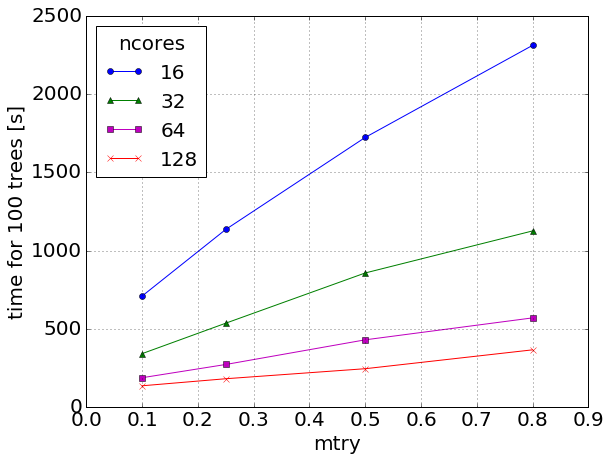
\includegraphics[totalheight=5cm]{../plos16/figs/mtry_cpu.png} 
      \caption{Time in seconds to build 100 trees for different mtry fractions. } 
      \label{figure:synthetictiming.a} 
      \vspace{4ex}
    \end{subfigure} 
    \hfill
    \begin{subfigure}[b]{0.45\linewidth}
      \centering
      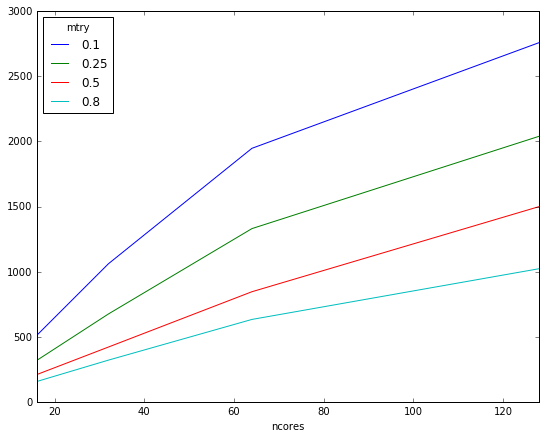
\includegraphics[totalheight=5cm]{../plos16/figs/cpu_mtry_trees_per_hour.png}
      \caption{Number of trees build per hour when using a growing number of CPU cores.}
      \label{figure:synthetictiming.b}
      \vspace{4ex}
    \end{subfigure} 
\end{figure}


\begin{figure}[tbhp]
    \caption{\textbf{Scalablity of the Wide Random Forest on synthetic datasets with varying number of samples and variables.}}
    \label{figure:synth2}
    \begin{subfigure}[b]{0.45\linewidth}
      \centering
      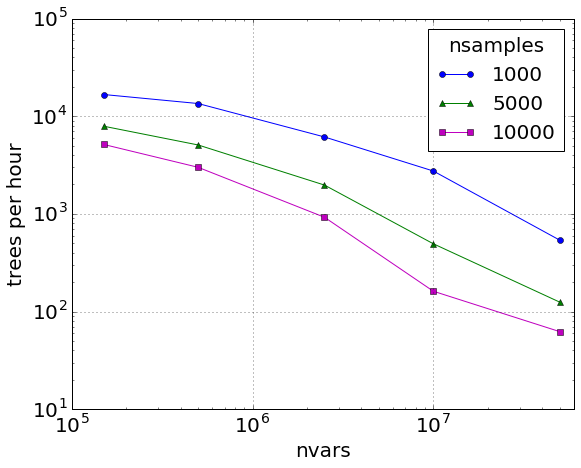
\includegraphics[totalheight=5cm]{../plos16/figs/nvars_nsamples.png} 
      \caption{Number of trees build per hour when growing number of variables.} 
      \label{figure:synth2.a} 
      \vspace{4ex}
    \end{subfigure} 
    \begin{subfigure}[b]{0.45\linewidth}
      \centering
      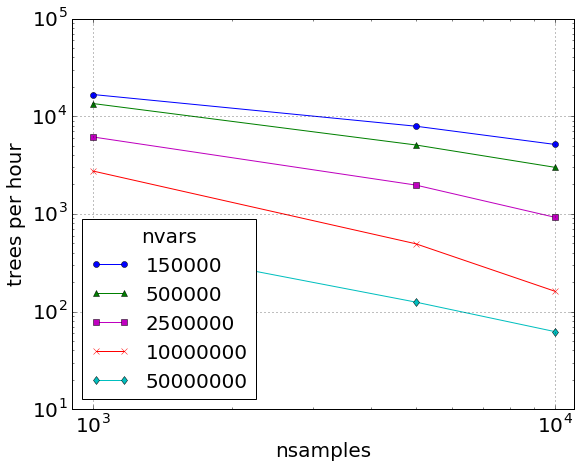
\includegraphics[totalheight=5cm]{../plos16/figs/nsamples_nvars.png}
      \caption{Number of trees build per hour when growing number of samples.}
    \label{figure:synth2.b}
    \vspace{4ex}
  \end{subfigure}
\end{figure}

\subsection{Exploring theoretical recovery rate of wide data}

 Donoho and Tanner \cite{Donoho.and.Tanner.2009} give a ``universal phase change'' result that has applications in a
 large number of areas including variable selection in high dimensions. Consider
 Fig~\ref{figure:phase-diagram-equivalence.png} which shows the region where a model can recover the important variables,
 plotted as a function of $\delta = n/p$ and $\rho =k/n$ (where $k$ is the number of significant variables). There is a
 distinct boundary, shown empirically and also based on arguments from combinatorial geometry, to the region where we can
 reliably recover significant variables.  \cite{Donoho.and.Stodden.2006} investigate the behavior of a number of
 regression approaches for variable selection (LARS, Lasso and forward stepwise) and make the point that above the
 phase-transition line variable recovery is still possible by a combinatorial approach.

 It is not surprising that that it is more difficult to recover the signal variable in the upper-left area of the figure,
 as the problem is both under-determined and sparse. What is surprising is the connection with arguments from
 combinatorial geometry. This suggests that we are seeing a universal rule rather than an implementation issue. As
 CursedForest is designed for extremely large numbers of variables it is likely to be operating in difficult regions of
 the figure where the ratio $\delta = n/p$ is small.


 We note several things here:
 \begin{itemize}
 \item the Donoho-Tanner phase transition arises in recovering the $\beta$ in data generated by a
   linear model. However, in a decision tree (random forest) there is no notion of estimating the $\beta$
 \item A decision tree (random forest) is a heuristic search. It may recover a relationship in the space of the
   combinatorial search.
 \end{itemize}

 The existence of the  Donoho-Tanner phase transition is a salutary warning. There are likely to be limits, both
 computational and logical, to the recovery of signals from noisy data. CursedForest  is a contribution to addressing the
 practical limits but the logical limits will still apply. However in the case of data that is both big and wide,
 CursedForest and other VariantSpark methods may provide a useful tool.


 \begin{figure}[tbhp] 
     \caption{\textbf{The Donoho-Tanner phase chage diagram.}}
     \centering
     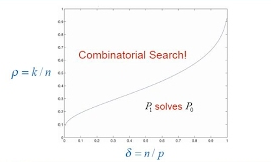
\includegraphics[totalheight=6cm]{../plos16/figs/phase.png} 
     \label{figure:phase-diagram-equivalence.png} 
     \vspace{4ex}
 \end{figure}

\begin{figure}[tbhp] 
    \begin{subfigure}[b]{0.45\linewidth}
      \centering
      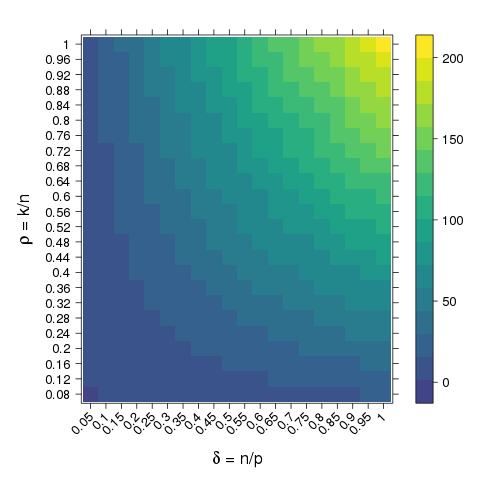
\includegraphics[totalheight=6cm]{../plos16/figs/k.png}
      \caption{$k$}
      \label{figure:k.png}
    \end{subfigure} 
    \begin{subfigure}[b]{0.45\linewidth}
      \centering
      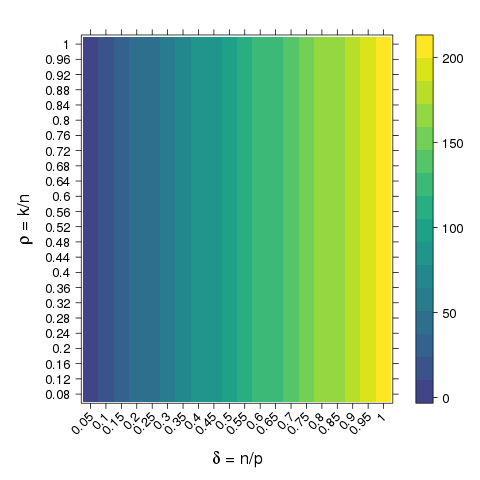
\includegraphics[totalheight=6cm]{../plos16/figs/n.png}
      \caption{$n$}
      \label{figure:n.png}
    \end{subfigure} 
    \caption{The simulation in \protect{\cite{Donoho.and.Stodden.2006}} considers $\delta = n/p$ and $\rho =k/n$. Here we plot the
      space of $\{ \delta, \rho$\}, colored  by the parameters $n$ and $k$}
\end{figure}

\subsection{Biological data}
We apply CursedForest to two biological datasets. Firstly, the 1000 genomes project to test its classification accuracy and secondly, to a bone mineral density dataset to demonstrate a GWAS-style analysis.
We training CursedForest on the 1000 genomes dataset, which consists of 2,504 samples with 81,047,467 features each to predict the ethnicity from genomic profiles. CursedForest achieves an out of bag error of OOB=0.01 and completes in 36 min 54 seconds, demonstrating its capability to run on population-scale cohorts of real world applications.
Next we perform feature selection on over 7.2 million genomic variants and identify the
locations associated with Bone Mineral Density (BMD) in a previously published GWAS dataset~\cite{Duncan.2011}. We faithfully recover 5 known BMD genes that were previously identified in GWAS studies, however also find two probable new associations that were previously only suggestive. This demonstrates the utility of our approach as well as the ability to amplify signal by taking SNP interactions into account rather than limiting the analysis to individual strong responders. 

\section{Conclusion}
We have demonstrated that using a different parallelization model can extend random forests to the case of an
extremely large number of variables. We have treated the case of variable selection in a $p >> n$ model, where most of
the variables are uninformative, and have demonstrated the utility of the model for large GWAS datasets. By comparing
this implementation to other implementations (including those optimized for large datasets) we have demonstrated the
utility of this approach.


\bibliographystyle{plain}
\bibliography{../plos16/CursedForest}

\end{document}  